% !TeX root =../../main.tex

\chapter{Introduction} \label{ch:introduction}


\section{Motivations and Challenges}
Software systems usually suffer from various kinds of vulnerabilities and weaknesses. These vulnerabilities can cause huge catastrophes from financial property loss to massive personnel casualty. For example, \emph{Heartbleed} (CVE-2014-0160)~\cite{heartbleed} is a critical vulnerability caused by an implementation defect in the widely used OpenSSL cryptographic software library which can compromise the integrity of communications across the entire Web. Further, it is reported that this may also affect the internal networks of enterprise in the coming years due to the fact that most enterprises do not have a good handle on the SSL encrypted services. Other software weaknesses may lead to more direct tragedies which lead to deaths. For example, the aircraft accident of Ethiopian Airlines Flight 302 in the late 2018 is high likely due to the improper functionality of the Maneuvering Characteristics Augmentation System (MCAS) from Boeing 737 Max~\cite{boeing_Ethiopian}. 153 lives were lost during this accident, including 149 passengers and 8 crew. Ironically, MCAS is designed to keep the balance of the airplane. The same Boeing 737 Max jet led to totally 189 people's death during Lion Air Flight 610 in 2019, which is also reported to result from the functionality of MCAS.

One interesting phenomenon needs to pay attention to is that it is usually a long time from \emph{the point that the vulnerability was introduced} to \emph{the point when the corresponding software was fully upgraded to the patched versions}. According to ``Vulnerability Review 2018 -- Global Trends''~\cite{vul_flexera18}, only 86\% vulnerabilities had a patch available on the day of disclosure in 2017, while in 2016 this percentage was 81\%. It is worth noting that some vendors choose to issue major product releases only. For the Heartbleed case, it is also interesting that this vulnerability was introduced in 2012 while was not discovered until 2 years later in 2014. Worse still, it also remains unknown when all the mainstream services will be upgraded to get grid of this vulnerability eventually. For the Boing 737 Max case, it is even unclear whether there is a solution for the remedy at all, despite the fact that its first flight was January, 2016, which has passed 3 years.

To avoid the damages brought by the software defects, it is favorable to \emph{disclose these vulnerabilities as early as possible and fix them immediately}. However, the vulnerability root causes essentially vary in different levels, including systematic level designing defects, as well as implementation level program crashes, etc. This poses significant challenges to secure these systems. Two widely applied approaches are \emph{testing} and \emph{verification}~\cite{Hailpern:2002:SDT:1660992.1660994,Felderer:2016:MST:2904681.2904685,mc-at}. However, neither of them can comprehensively reveal security defects in the software systems effectively and efficiently. On one hand, verification systematically proves the absence of certain defects in the system. Due to its complexity nature, the programs or the systems that are verified are usually abstracted in an intermediate representation and the focus is a relative higher level security guarantee. However modeling the system correctly usually takes considerable time and the applied abstraction may miss subtle issues in the implementation. On the other hand, testing is effective in practice to reveal implementation vulnerabilities with test cases; it checks the different functionalities of the target program by considering different application scenarios. However, there is no guarantee that the system is free of vulnerabilities that are not covered by these tests; more importantly, it usually lacks the insight of the higher level design vulnerabilities. For example, although it is possible for fuzz testing to discover multiple crashes in Android core libraries, it usually cannot reveal certain categories of various security issues regarding privacy at the application framework level and the applications built on top of it~\cite{Enck:2009:UAS:1512148.1512324,Ernst:2014}. In fact, it is almost impossible for testing techniques to detect certain security issues in Android due to its designing flaw~\cite{url:android-flaw}.

\begin{figure}[t]
	\begin{center}
		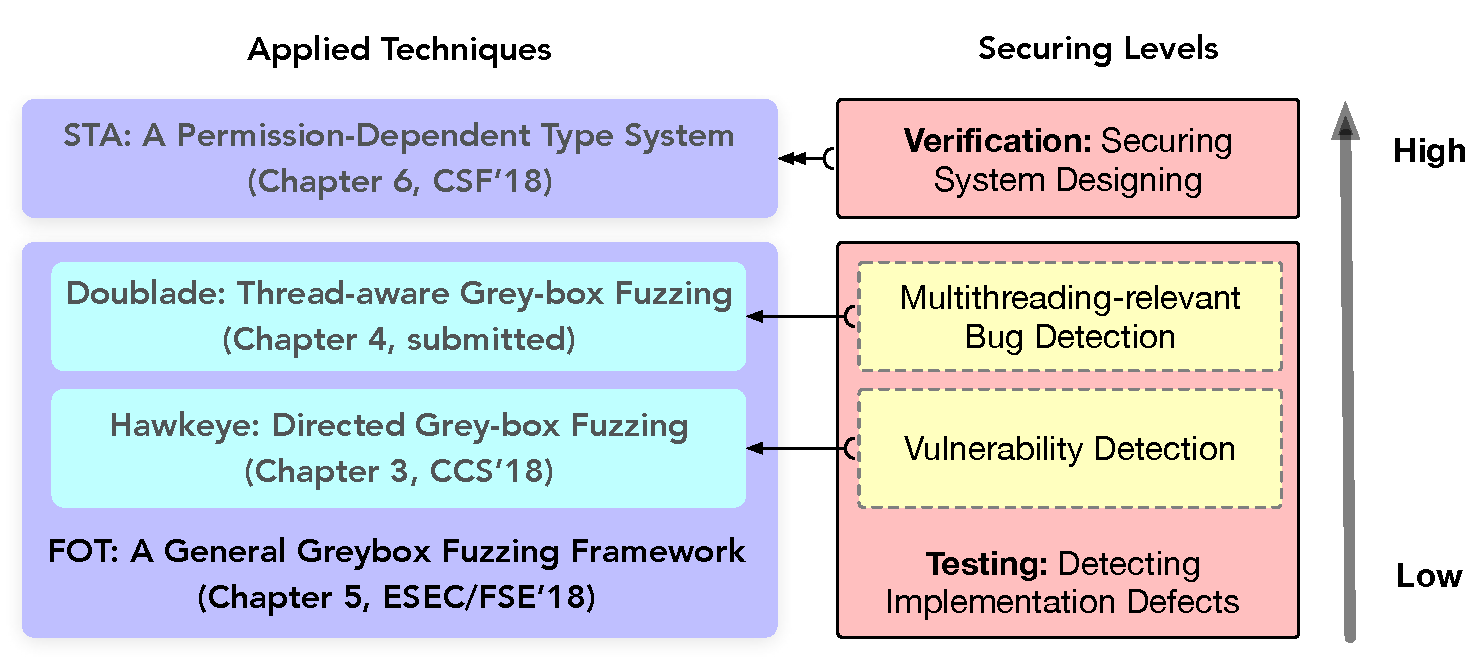
\includegraphics[width=0.98\textwidth]{res/contributions_new}
		\caption{Main work of this thesis and the relations among its counterparts}
		\label{fig:works}
	\end{center}
\end{figure}


\section{Main Work}

My work attempts to secure these systems by applying both testing and verification techniques for different levels of vulnerability detection.  Figure~\ref{fig:works} depicts the major parts of my work as well as their relations between different parts. For lower level implementation vulnerabilities, we rely on testing: this includes detecting vulnerabilities caused by buffer-overflow, use-after-free, etc --- this lies in the lowest in the vulnerability hierarchy, as well as detecting relatively higher level concurrency-relevant bugs such as data-races or vulnerabilities in the multithreading environment. For higher level designing defects, we rely on verification, our target is the permission based access control defects which cannot be (exhaustively) revealed by testing.

As to testing, we apply the greybox fuzzing approaches to reveal those \emph{implementation vulnerabilities}.
Firstly, in order to guide the fuzzing procedure to \emph{certain specific program locations}, we propose \dFOT, which can be applied to scenarios such as patching testing, crash reproduction, etc. We summarize four key properties that are considered important to the guidance: the robust directedness mechanism, the lightweight yet effective integration with static analysis, the optimized seed prioritization and scheduling strategies, as well as adaptive strategies across fuzzing states. 
Secondly, in order to improve the efficiency of fuzzing multi-threaded programs, we propose \mtfuzz, a directed greybox fuzzer which utilizes the thread-aware analyses to increase the quality of the generated seeds. \mtfuzz provides the thread-interleaving feedback by providing a novel stratified exploration oriented instrumentation, together with the threading context information and the thread scheduling intervention that diversifies the actual interleaving.
In addition, to integrate these different state-of-the-art fuzzing techniques, we build a general-purpose greybox fuzzing framework called \emph{Fuzzing Orchestration Toolkit}~\cite{fse18-fot} (a.k.a. \FOT). This framework aims to be \emph{versatile}, \emph{configurable}, and \emph{extensible}. It is versatile since it has integrated and will integrate various greybox fuzzing techniques~\cite{Bohme:2016:CGF,Bohme:2017:DGF,redqueen,CollAFL,Angora,fuzz_survey,junjie:2017sp:skyfire,LiCMLLT17,superion,Wen2020MemLock,Wang2020Typestate}. It is configurable in the sense that it provides several builtin strategies which allow easy customization for the fuzzing procedure. It is also extensible in the sense that it provides fruitful interfaces for easy integration with new techniques. Both \dFOT and \mtfuzz are built on top of \FOT, which heavily rely on the latter's static analysis integration.

In order to secure the higher level designing defects such as information leakage in Android system, we propose a permission-dependent security type system to rigorously certify that the underlying system is free of these vulnerabilities. The novelty of the proposed type system is that we designed a type merging operator that allows for permission-dependent typing. We proved the soundness of the type system in terms of \emph{non-interference}, in which we formally assure no information leakage in the system as long as the security type checking is passed. We also provided a set of type inference rules that are guaranteed to be decidable within a finite number of steps. In addition, we implemented a prototype of the type system which can type check the information leakage issues in Android.

With these applied approaches, we aim to provide a comprehensive solution, which ranges in different levels of vulnerability detection, to securing various software systems such as Linux or Android.

\section{Contributions of the Thesis}
The contributions of the thesis is as follows:
\begin{enumerate}
	\item We proposed a principled directed greybox fuzzing technique, \dFOT, to allow for fuzzing on specific program target locations. \dFOT provides the robust directedness mechanism, integrates with a static analysis to calculate the directedness utilities, optimizes seed prioritization and scheduling, and applies adaptive mutation strategies across different distance states. This significantly improves the fuzzing effectiveness on the specified program target locations.
	\item We proposed a thread-aware fuzzing technique, \mtfuzz, which significantly improved the effectiveness of fuzzing on multi-threaded programs. \mtfuzz utilizes the thread-aware analysis and applies three categories of instrumentation to explore thread-interleavings,  improve the thread-scheduling diversities across executions, and consider threading context; based on the feedback provided by the instrumentations, \mtfuzz generates more valuable seeds that can significantly help reveal multithreading-relevant bugs.
	\item We provided a greybox fuzzing framework, \FOT, which is versatile in its configurability and extensibility. Based on this, we have integrated several fuzzing techniques, including \dFOT and \mtfuzz, and successfully detected more than 200 vulnerabilities in real-world open source programs, among which 51 have been assigned CVE IDs.
	\item We provided a permission-dependent type system that precisely enforces access control based on the permission authentication mechanism on Android and proved its soundness in term of the non-interference property. We also provided a series of decidable type inference rules to assist the type checking. Based on the type system, we implemented a prototype that stresses information leakage issues in Android system.
\end{enumerate}


\section{List of Materials Related to the Thesis}
\begin{enumerate}
	\item \myname, Yuekang Li, Bihuan Chen, Yinxing Xue, Yang Liu, ``FOT: A Versatile, Configurable, Extensible Fuzzing Framework'', ESEC/FSE '18, Proceedings of the 2018 26th ACM Joint Meeting on European Software Engineering Conference and Symposium on the Foundations of Software Engineering, Pages 867-870, \url{http://doi.acm.org/10.1145/3236024.3264593}, DOI: 10.1145/3236024.3264593.
	\item \myname, Yinxing Xue, Yuekang Li, Bihuan Chen, Xiaofei Xie, Xiuheng Wu, Yang Liu, ``Hawkeye: Towards a Desired Directed Greybox Fuzzer'', CCS'18, Proceedings of the 2018 ACM SIGSAC Conference on Computer and Communications Security, Pages 2095-2108, \url{http://doi.acm.org/10.1145/3243734.3243849}, DOI: 10.1145/3243734.3243849.
	\item \myname, Shengjian Guo, Yinxing Xue, Yulei Sui, Cen Zhang, Yuekang Li, Haijun Wang, Yang Liu, ``\mtfuzz: Thread-aware Grey-box Fuzzing for Effective Bug Hunting in Multithreaded Programs'', submitted.
	\item \myname, Alwen Tiu, Zhiwu Xu, Yang Liu, ``A Permission-Dependent Type System for Secure Information Flow Analysis'', 2018 IEEE 31st Computer Security Foundations Symposium (CSF'18), Oxford, 2018, pp. 218-232. \url{https://doi.org/10.1109/CSF.2018.00023}, DOI: 10.1109/CSF.2018.00023. A technical report is available at \url{https://arxiv.org/abs/1709.09623}.
\end{enumerate}

\section{Outline of the Thesis}

The rest of the thesis is organized as follows.

Chapter~\ref{ch:preliminaries} describes the terminologies and preliminaries throughout this paper. Chapter~\ref{ch:dfot} explains our directed greybox fuzzer \dFOT; \dFOT is our attempt to guide the fuzzing process to specific program target locations. Chapter~\ref{ch:mtfuzz} describes \mtfuzz, which aims to enhance the fuzzing effectiveness on multithreaded programs. Chapter~\ref{ch:fot} introduces our greybox fuzzing framework, \FOT, which has integrated multiple greybox fuzzing techniques.  Chapter~\ref{ch:sta} describes our attempt to secure software systems based on verification, which applies a permission-dependent type system to enforce the non-interference property that prevents information leakage in an Android system. Chapter~\ref{ch:conclusion} discusses my reflection on the testing and verification based techniques and finally concludes the thesis.